\documentclass[conference]{IEEEtran}
\IEEEoverridecommandlockouts
% The preceding line is only needed to identify funding in the first footnote. If that is unneeded, please comment it out.
\usepackage[acronym,toc]{glossaries}
\usepackage{cite}

\usepackage[T1]{fontenc}

\usepackage{booktabs}
\usepackage{colortbl}
\usepackage{xcolor}
\usepackage{multirow}

\usepackage[main=english,portuguese]{babel}
\usepackage{ucs}
\usepackage[utf8x]{inputenc}

\usepackage{pdfpages}
\usepackage{blindtext}
\usepackage{adjustbox}
\usepackage{comment}
\usepackage{siunitx}
\usepackage{graphicx}
\definecolor{lightgray}{RGB}{236, 238, 237}
\definecolor{peach}{RGB}{255, 190, 153}
\definecolor{blue}{RGB}{55, 104, 183}
\definecolor{navyblue}{RGB}{9, 7, 54}
\definecolor{lightorange}{RGB}{252, 221, 191}
\usepackage{listings}
\lstset{ 
    language=bash, % choose the language of the code
    basicstyle=\fontfamily{pcr}\selectfont\tiny\color{blue},
    keywordstyle=\color{navyblue}\bfseries, % style for keywords
    numbers=none, % where to put the line-numbers
    numberstyle=\tiny, % the size of the fonts that are used for the line-numbers     
    backgroundcolor=\color{white},
    showspaces=false, % show spaces adding particular underscores
    showstringspaces=false, % underline spaces within strings
    showtabs=false, % show tabs within strings adding particular underscores
    frame=single, % adds a frame around the code
    tabsize=2, % sets default tabsize to 2 spaces
    captionpos=b, % sets the caption-position to bottom
    breaklines=true, % sets automatic line breaking
    breakatwhitespace=false, 
}
\usepackage{amsmath}
\usepackage{amssymb}
\usepackage{float}

\newacronym{3GPP}{3GPP}{$3^{rd}$ Generation Partnership Project}
\newacronym{4G}{4G}{Fourth Generation}
\newacronym{AI}{AI}{Artificial Intelligence}	
\newacronym{AMPS}{AMPS}{Advanced Mobile Phone System}	
\newacronym{API}{API}{Application Programming Interface}	
\newacronym{AR}{AR}{Augmented Reality}	
\newacronym{CLI}{CLI}{Command Line Interface}
\newacronym{CM}{CM}{Configuration Management}	
\newacronym{DevOps}{DevOps}{Development and Systems Operation}
\newacronym{DOM}{DOM}{Document Object Model}	
\newacronym{DRY}{DRY}{Don't Repeat Yourself}	
\newacronym{DT}{DT}{Drive-test}	
\newacronym{EM}{EM}{Energy Management}	
\newacronym{ERD}{ERD}{Entity Relationship Diagram}
\newacronym{GSM}{GSM}{Global System for Mobile Communications}	
\newacronym{HTML}{HTML}{HyperText Markup Language}
\newacronym{HTTP}{HTTP}{Hypertext Transfer Protocol}	
\newacronym{KPI}{KPI}{Key Performance Indicators}	
\newacronym{LTE}{LTE}{Long Term Evolution}
\newacronym{LXC}{LXC}{Linux Containers}
\newacronym{ML}{ML}{Machine Learning}	
\newacronym{MVC}{MVC}{Model-View-Controller}	
\newacronym{MVT}{MVT}{Model-View-Template}	
\newacronym{ORM}{ORM}{Object-Relational Mapping}	
\newacronym{OS}{OS}{Operating System}
\newacronym{PaaS}{PaaS}{Platform as a Service}
\newacronym{PID}{PID}{Process Unique Identifier}
\newacronym{PM}{PM}{Performance Management}	
\newacronym{QoE}{QoE}{Quality Of Experience}	
\newacronym{RINNOS}{RINNOS}{Research Innovation Studio}	
\newacronym{RQ}{RQ}{Redis Queue}
\newacronym{RTT}{RTT}{Round Trip Time}
\newacronym{SLA}{SLA}{Service Level Agreement}	
\newacronym{SMS}{SMS}{Short Message System}	
\newacronym{SP}{SP}{Service Providers}	
\newacronym{STDIN}{STDIN}{Standard Input}
\newacronym{STDOUT}{STDOUT}{Standard Output}
\newacronym{UI}{UI}{User Interface}
\newacronym{UID}{UID}{Unique Identifier}
\newacronym{UMTS}{UMTS}{Universal Mobile Telecommunications Service}
\newacronym{VM}{VM}{Virtual Machines}
\newacronym{VMM}{VMM}{Virtual Machine Monitor}
\newacronym{VR}{VR}{Virtual Reality}	
\newacronym{VoIP}{VoIP}{Voice Over IP}	
\newacronym{WPF}{WPF}{Windows Presentation Foundation}
\newacronym{WSL}{WSL}{Windows Subsystem for Linux}


\newacronym{IST}{IST}{Instituto Superior T\'ecnico}
\newacronym{UE}{UE}{User Equipment}
\newacronym{IoT}{IoT}{Internet of Things}
\newacronym{CC}{CC}{Cloud Computing}
\newacronym{QoS}{QoS}{Quality-of-Service}
\newacronym{MEC}{MEC}{Mobile Edge Computing}
\newacronym{ETSI}{ETSI}{European Telecommunications  Standards  Institute}
\newacronym{MDP}{MDP}{Markov Decision Process}
\newacronym{DNN}{DNN}{Deep Neural Networks}
\newacronym{RL}{RL}{Reinforcement Learning}
\newacronym{DRL}{DRL}{Deep Reinforcement Learning}
\newacronym{FC}{FC}{Fog Computing}
\newacronym{SDN}{SDN}{Software Defined Network}
\newacronym{ISG}{ISG}{Industry Specification Group}
\newacronym{RAN}{RAN}{Radio Access Network}
\newacronym{SCC}{SCC}{Small Cell Cloud}
\newacronym{SCM}{SCM}{Small Cell Manager}
\newacronym{MMC}{MMC}{Mobile Micro Cloud}
\newacronym{MobiScud}{MobiScud}{Fast  Moving  Personal  Cloud}
\newacronym{MC}{MC}{MobiScud Control}
\newacronym{FMC}{FMC}{Follow  Me  Cloud}
\newacronym{SCeNBs}{SCeNBs}{Small Cells}
\newacronym{eNB}{eNB}{Wireless Base Station}
\newacronym{CN}{CN}{Core Network}
\newacronym{NFV}{NFV}{Network Function Virtualization}
\newacronym{POMDP}{POMDP}{Partially  Observable  Markov  Decision  Process}
\newacronym{ANNs}{ANNs}{Artificial Neural Networks}
\newacronym{DQN}{DQN}{Deep Q-Network}
\newacronym{CNNs}{CNNs}{Convolutional Neural Networks}
\newacronym{RNNs}{RNNs}{Recurrent Neural Networks}
\newacronym{DDQN}{DDQN}{Double Deep Q-Network}
\newacronym{TD}{TD}{Temporal Difference}
\newacronym{Dueling DQN}{Dueling DQN}{Dueling Deep Q-Network}
\newacronym{A3C}{A3C}{Asynchronous Advantage Actor-Critic}
\newacronym{A2C}{A2C}{Advantage Actor-Critic}
\newacronym{AGA}{AGA}{Adaptive Genetic Algorithm}
\newacronym{IaaS}{IaaS}{Infrastructure as a Service}
\newacronym{VMs}{VMs}{Virtual Machines}
\newacronym{GPU}{GPU}{Graphics Processing Unit}
\newacronym{CPU}{CPU}{Central Processing Unit}
\newacronym{DRQN}{DRQN}{Deep Recurrent Q-Network}

\begin{document}

\title{Task offloading optimization in Mobile Edge Computing based on Deep Reinforcement Learning}

\author{\IEEEauthorblockN{C. Silva\textsuperscript{1}}
\IEEEauthorblockA{\textsuperscript{1}\textit{Instituto Superior Técnico,} \\
University of Lisbon\\
Lisbon, Portugal\\
carlos.m.a.silva@tecnico.ulisboa.pt}}

\maketitle

\begin{abstract}
The \acrfull{CC} paradigm has risen in recent years as a solution to a need for computation and battery constrained \acrfull{UE} to run increasingly intensive computation tasks. Nevertheless, given the centralized nature of the \acrshort{CC} paradigm, this option introduces significant network congestion problems and unpredictable communication delays not suitable for real-time applications. In order to cope with these problems, the \acrfull{MEC} concept has been introduced, which proposes to bring computation resources closer to the edge of the mobile networks in a distributed way. However, given that these edge computation resources are limited, this paradigm comes with its set of challenges that need to be solved in order to make it viable. This work proposes to innovate by presenting a network management agent capable of making offloading decisions from a heterogeneous network of \acrshort{UE}s to a heterogeneous network of \acrshort{MEC} servers. This agent represents an orchestrator of a group of 5G \acrfull{SCeNBs}, enhanced with computation and storage capabilities. In order to solve this high complexity problem, an \acrfull{A2C} agent is implemented and tested against several baselines. The proposed solution is shown to beat the baselines by making intelligent decisions taking into
account computation, battery, delay and communication constraints ignored by the baselines. The solution is also shown to be scalable, data-efficient, robust, stable and adjustable to address not only overall system performance but to take into account the worst-case scenario.
\end{abstract}

\begin{IEEEkeywords}
Mobile Edge Computing, Computation Offloading, Energy and Performance Optimization, Delay Sensitivity, Deep Reinforcement Learning, Cloud Computing
\end{IEEEkeywords}

\section{Introduction}

\noindent There has been a continuous exponential increase in the number of \acrfull{UE}, such as smartphones, laptops and \acrfull{IoT} devices. Their need to run ever more complex applications, given their energy and computation constrained environment, has led to the rise of \acrfull{CC} as an alternative to offload computation and storage needs. In the \acrshort{CC} paradigm, computation resources are located in centralized data centers that can be considered infinite. This paradigm brings several advantages \cite{SHAKARAMI2020107496}: 
\begin{enumerate}
    \item By offloading computation, it extends the battery life of \acrshort{UE}; 
    \item Enables computationally complex applications intractable with \acrshort{UE} computation capabilities;
    \item Provides seemingly unlimited storage capacity.
\end{enumerate}
However, there are also shortcomings. The two main problems introduced by this paradigm are: 
\begin{enumerate}
    \item The distance from \acrshort{UE}s to these servers introduces an unpredictable communication latency that makes some delay-constrained applications unviable;
    \item  This increase in \acrshort{UE}s and their communication needs with \acrshort{CC} servers leads to ever more congested network links decreasing \acrfull{QoS} for everyone in the network.
\end{enumerate}

\par
These shortcomings gave rise to a new emerging concept known as \acrfull{MEC}. The main idea of \acrshort{MEC} is to bring computation resources closer to the edge of the mobile network enabling offloading of complex computation tasks with strict delay requirements. As defined by the \acrfull{ETSI} in \cite{MECspec}, this can be achieved by allocating computing nodes at the network's edge in a fully distributed manner to reduce communication overhead and execution delay for \acrshort{UE}s.

\subsection{Motivation}
\noindent Edge computing nodes come with limited radio, storage and computational resources, which raise three main challenges \cite{SHAKARAMI2020107496}:
\begin{itemize}
    \item The \textbf{decision of which computing tasks} are profitable for the \acrshort{UE} to offload to the \acrshort{MEC} servers in terms of energy consumption and execution delay.
    \item How to efficiently \textbf{allocate the limited computation resources} within the \acrshort{MEC} servers in order to minimize response delay and load balance the computing resources and communication links.
    \item \textbf{Mobility management} to guarantee \acrshort{MEC} service continuity and efficiency for \acrshort{UE}s roaming the network.
\end{itemize}

Given the heterogeneous and stochastic nature of network topologies, traditional optimization techniques lack the scalability and adaptability to deal with unknown network conditions. Recent breakthroughs in machine learning algorithms, showcasing their ability to solve and adapt to complex problems previously thought impossible to be solved by a computer, led many researchers to explore applying these methods to the \acrshort{MEC} challenges.
\par
The problem of making offloading and resource allocation decisions in \acrshort{MEC} can be simulated and performance benchmarks are easily defined. This makes their definition as a \acrfull{MDP} straightforward and allows the use of promising algorithms, like \acrfull{DNN} trained using \acrfull{RL} or \acrfull{DRL} algorithms for short. 

\subsection{Contributions}
\noindent The main contributions of this work are:
\begin{itemize}
    \item The implementation of an open-source, \acrshort{A2C} agent, capable of making intelligent offloading decisions that take into account battery, computation and communication constraints overperforming the baselines in a heterogeneous network of several \acrshort{UE}s and \acrshort{MEC} servers;
    \item The release of an open-source realistic network simulation environment as an OpenAI Gym, \cite{opengym}, environment. Allowing for easy experimentation with different \acrshort{DRL} algorithms;
\end{itemize}

\section{Related Work}

\subsection{Overview of \acrshort{MEC} architectures} \label{section:MECarch}

\noindent One of the first efforts to bring computation resources closer to the edge was the cloudlet concept presented in \cite{cloudlet}. The main idea behind it was to allocate powerful computers at WiFi hotspots that could sell their \acrfull{IaaS} through the use of \acrfull{VMs}.

Another concept to bring computation closer to \acrshort{UE}s is the idea of an \emph{ad-hoc} cloud like the one presented in \cite{adhoc}. The idea proposes that the computation power of a network of non-exclusive and sporadically available hosts can be harvested and abstracted as a service to which \acrshort{UE}s can offload their computational needs.

Finally, the \acrfull{MEC} concept presented by the \acrfull{ISG} within the \acrfull{ETSI} in \cite{MECspec} is focused on integrating computation resources within the \acrfull{RAN} in very close proximity to mobile subscribers.

As presented in paper \cite{SHAKARAMI2020107496}, several \acrshort{MEC} architectures have been proposed in order to integrate and manage computation resources at the \acrshort{RAN} level, such as \acrfull{SCC} \cite{smallcellcloud}, \acrfull{MMC} \cite{mmcloud}, \acrfull{MobiScud} \cite{MobiScud}, \acrfull{FMC} \cite{fmcloud} and CONCERT \cite{CONCERT}.

\subsection{Reinforcement Learning (RL)} \label{section:RL}
\noindent There are three main machine learning paradigms, supervised learning, unsupervised learning and reinforcement learning. While supervised learning needs a lot of labeled input/output data and unsupervised learning learns patterns from unlabeled data, \acrfull{RL} is used in problems where an agent learns to solve a closed-loop problem by changing its future actions based on a reward resulting from its actions on the environment and its effects on its state.

This paradigm has shown great potential in solving environments that can be simulated and easily benchmarked, which is the reason most research on \acrshort{RL} is made by solving video games, which offer a perfect environment in terms of reproducibility, easy simulation and baked in benchmarks that can be used to compute a reward signal (points, levels, etc.).

Several algorithms have been proposed from \acrfull{DQN} in \cite{DQN}, \acrfull{DDQN} in \cite{doubleDQN}, Dueling Deep Q-Network (Dueling DQN) in \cite{duelingDQN} and \acrfull{A3C} in \cite{a3c}.

\subsection{Exploitation vs Exploration} \label{section:EE}
\noindent One major challenge a \acrshort{RL} agent faces is the exploration vs exploitation dilemma. Given a fixed set of resources that must be allocated between competing choices in a way that maximizes expected reward in an unknown transition probability and reward signal environment, the agent must choose to perform actions that exploit known strategies versus performing unknown actions to explore the environment for better strategies. These types of problems have been studied extensively as multi-armed bandit problems.

In order to solve this problem several algorithms have been proposed from $\epsilon$-greedy algorithm, Boltzmann exploration in \cite{boltz} and \acrfull{AGA} in \cite{AGAcrypto}.

\section{Problem statement}

\noindent The goal of this thesis is the design of a management agent capable of making offloading decisions from a heterogeneous network of \acrshort{UE}s to a heterogeneous network of \acrshort{MEC} servers. This work proposes to innovate by presenting a more complete system and exploring a network topology not present in related works. The proposed network manager could be seen as the conductor in the CONCERT architecture proposed in \cite{CONCERT} or the small cell manager in the \acrshort{SCC} architecture, \cite{SESAM}. This manager would be deployed locally and would manage a group of $M$ \acrshort{MEC} servers and $N$ \acrshort{UE}s making offloading decisions on which \acrshort{UE} tasks to compute locally, which tasks to offload and where tasks should be offloaded to. This decision should take into account communication delays, computation constraints and battery consumption.

Building upon the system presented in \cite{NUE1mec}, the proposed system plans address its shortcomings by:
\begin{itemize}
    \item Expanding the number of \acrshort{MEC} servers that must be orchestrated from one to $M$ servers, better representing a 5G network with several \acrshort{SCeNBs} enhanced with computation capabilities;
    \item Testing the management agent in a heterogeneous environment, with \acrshort{UE}s and \acrshort{MEC} servers of different computation capabilities;
    \item Taking into account the delay and energy cost of downloading the processed result from the \acrshort{MEC} server to the \acrshort{UE};
    \item Exploring modern \acrshort{DRL} algorithms to solve the increased complexity problem.
\end{itemize}

\subsection{System Model}
\noindent The proposed network model considers \emph{N} \acrshort{UE}s and \emph{M} \acrshort{MEC} servers, as represented in Figure \ref{proposed_network}. 

\begin{figure}[H]
  \centering
  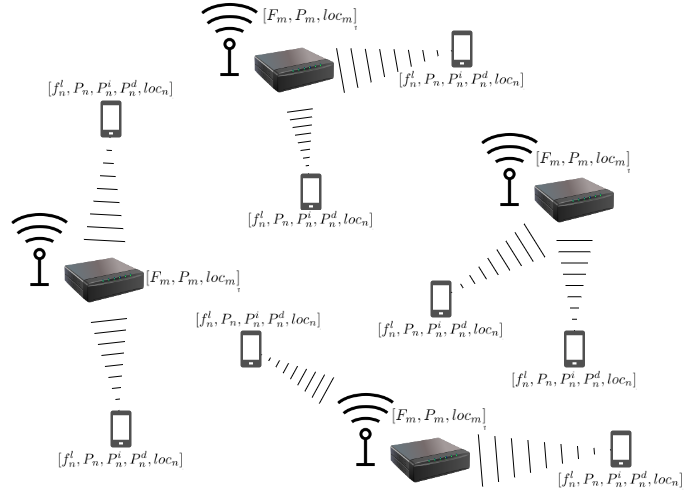
\includegraphics[width=\linewidth]{images/proposed_network.png}
  \caption{Proposed network model.} \label{proposed_network}
\end{figure}

The set of \acrshort{UE} is denoted as $\mathcal{N} = \{1, 2, ..., N\}$ while the set of \acrshort{MEC} servers can be denoted as $\mathcal{M} = \{1, 2, ..., M\}$. For simplicity \acrshort{MEC} servers are assumed to be connected to the power grid so their energy consumption is ignored.
\begin{itemize}
    \item Each \acrshort{UE}, $n \in \mathcal{N}$ can be described by its computing capacity, $f_n^l$ (\acrshort{CPU} cycles per second), transmit power, $P_n$, idle power consumption, $P^i_n$, download power consumption, $P_n^d$, and location, $loc_n = (x_n, y_n, z_n)$. The UE, $n$, can then be described by the vector, $u_n = [f_n^l, P_n, P_n^i, P_n^d, loc_n]$, and the system's \acrshort{UE}s can be defined as the vector $\mathcal{U} = [u_1, u_2, ..., u_n]$.

    \item Each \acrshort{MEC} server, $m \in \mathcal{M}$, can be described by its computing capacity, $F_m$ (\acrshort{CPU} cycles per second), its transmit power, $P_m$, and its location $loc_m = (x_n, y_n, z_n)$. The \acrshort{MEC} server, $m$, can then be described by the vector, $s_m = [F_m, P_m, loc_m]$ and the system's \acrshort{MEC} servers can be defined as the vector $\mathcal{S} = [s_1, s_2, ..., s_n]$.

    \item At each time step each \acrshort{UE} is assumed to have a computation task to be completed. This task can either be computed locally or offloaded to one of the available \acrshort{MEC} servers. The offloading decision of each computation task is denoted as $\alpha_n \in \{0, 1, ..., M\}$, where $\alpha_n = 0$ means local computation and $\alpha_n \in \mathcal{M}$ means offloading the task to \acrshort{MEC} server $m = \alpha_n$. The total offloading decision can be defined as the decision vector $\mathcal{A} = [\alpha_1, \alpha_2, ..., \alpha_N]$ with a decision for each task.

    \item Each computation task, $R_n$, can be defined by an input data amount, $B_n$ (bits), an output data amount, $B_d$ (bits), the total number of \acrshort{CPU} cycles required to compute it, $D_n$ and the importance weights of time and energy costs, $I_n^t$ and $I_n^e$. The importance weights of the task must satisfy $0 \leq I_n^t \leq 1$, $0 \leq I_n^e \leq 1$ and $I_n^t + I_n^e = 1$. The task, $R_n$, can then be described by the vector, $R_n = [B_n, B_d, D_n, I_n^t, I_n^e]$ and the system's tasks can be defined as the vector $\mathcal{R} = [R_1, R_2, ..., R_N]$.


\end{itemize}

If the network manager decides to compute the task, $R_n$, of \acrshort{UE} $n$ locally then a local computation model can be defined by a local execution delay $T_n^l$ and an energy consumption $E_n^l$:

\begin{equation}
    T_n^l = \frac{D_n}{f_n^l},
\end{equation}

\begin{equation}
    E_n^l = z_n D_n,
\end{equation}

where $z_n$ represents the energy consumption per \acrshort{CPU} cycle and is set to $z_n = 10^{-27}(f_n^l)^2$ according to practical observations made in \cite{energycons}.

Based on the computation delay and energy consumption of task, $R_n$, a local cost can be calculated according to:

\begin{equation}\label{localCost}
    C_n^l = I_n^t T_n^l + I_n^e E_n^l .
\end{equation}

If the network manager decides to offload the computation to the \acrshort{MEC} server $m = \alpha_n$, then the offload computation model can be defined by an upload delay, $T_{n,t}^m$, an upload energy consumption, $E_{n,t}^m$, an offload execution delay, $T_{n,p}^m$, an idle energy consumption, $E_{n,p}^m$, a download delay, $T_{n,d}^m$ and its corresponding download energy consumption, $E_{n,d}^m$.

Firstly, the \acrshort{UE} $n$ must upload the input data, $B_n$ from the task $R_n$ to the decided \acrshort{MEC} server $m$. This upload has an associated delay defined as:

\begin{equation} \label{transmission_delay}
    T_{n,t}^m = \frac{B_n}{r_u},
\end{equation}

where $r_u$ is the uplink rate of \acrshort{UE} $n$.

This upload has an associated energy consumption:

\begin{equation} \label{transmission_energy}
    E_{n,t}^m = P_n T_{n,t}^m = \frac{P_n B_n}{r_u} .
\end{equation}

After the data is uploaded the \acrshort{MEC} server then computes the task resulting in a offload execution delay:

\begin{equation} \label{processing_delay}
    T_{n,p}^m = \frac{D_n}{f_m} ,
\end{equation}

where $f_m$ is the amount of the \acrshort{MEC} server, $m$, computation capacity, $F_m$, allocated to the offloaded task. To simplify the system the computation capacity of a \acrshort{MEC} server is equally divided by all tasks offloaded to it:

\begin{equation}
    f_m = \frac{F_m}{N_m},
\end{equation}

where $N_m$ is the number of tasks offloaded to \acrshort{MEC} server, $m$.

While the \acrshort{UE} waits for the task to be computed it stays idle which has an associated energy consumption:

\begin{equation} \label{idle_energy}
    E_{n,p}^m = P_n^i T_{n,p}^m = \frac{P_n^i D_n}{f_m}.
\end{equation}

Finally the computation results are downloaded to the \acrshort{UE} $n$ with an associated delay:

\begin{equation} \label{download_delay}
    T_{n, d}^m = \frac{B_d}{r_d},
\end{equation}

where $B_d$ is the size of the computation output and $r_d$ is the download rate of \acrshort{UE} $n$.

This download step has an associated energy consumption that can be calculated according to:

\begin{equation} \label{download_energy}
    E_{n, d}^m = P_n^d T_{n, d}^m .
\end{equation}

By taking into account the delays defined in Equations (\ref{transmission_delay}), (\ref{processing_delay}) and (\ref{download_delay}), we can compute the total offload delay, $T_n^m$ as the sum of all delays:

\begin{equation}
    T_n^m = T_{n,t}^m + T_{n,p}^m + T_{n, d}^m .
\end{equation}

The total energy consumption of offloading to the \acrshort{MEC} server $m$, can be calculated by adding all energy consumptions defined in Equations (\ref{transmission_energy}), (\ref{idle_energy}) and (\ref{download_energy}):

\begin{equation}
    E_n^m = E_{n,t}^m + E_{n,p}^m + E_{n, d}^m .
\end{equation}

Based on the computation delay and energy consumption of offloading task $R_n$ to \acrshort{MEC} server $m$, a cost can be calculated according to:

\begin{equation}
    C_n^m = I_n^t T_n^m + I_n^e E_n^m .
\end{equation}

The cost of the offloading decision $\alpha_n \in \{0, 1, ..., M\}$ can be computed according to:

\begin{equation}
    C_n =
    \begin{cases}
        C_n^l & \alpha_n = 0             \\
        C_n^m & \alpha_n \in \mathcal{M}
    \end{cases} .
\end{equation}

The system's costs can be defined as the vector:

\begin{equation}
    \mathcal{C} = [C_1, C_2, ..., C_N].
\end{equation}


The mean cost of the \acrshort{MEC} system at each iteration can then be defined as:

\begin{equation} \label{C_mean}
    C_{mean} = \frac{\sum\limits_{n=1}^N C_n}{N}.
\end{equation}

The worst-case cost of the \acrshort{MEC} system at each iteration can then be defined as:

\begin{equation}
    C_{max} = \max \ \mathcal{C}.
\end{equation}

This corresponds to the \acrshort{UE} that has the highest cost at each iteration.

\subsection{Problem formulation}
\noindent The offloading decision needs to be formulated in a way that can both optimize overall system performance while considering the worst-case serviced \acrshort{UE}.

Given this, the weighted cost at each iteration can be defined as:

\begin{equation} \label{cost_function}
    C = W_{mean}*C_{mean} + W_{max}*C_{max}.
\end{equation}

By picking the importance weights of the costs that satisfy:
\begin{align*}
    0 \leq W_{mean} \leq 1, \\
    0 \leq W_{max} \leq 1,  \\
    W_{mean} + W_{max} = 1.
\end{align*}

The priorities of the system can be adjusted to satisfy both overall system performance and consider the worst-case cost of the system.

The optimization function can then be defined with the objective of finding the offloading decision vector $\mathcal{A} = [\alpha_1, \alpha_2, ..., \alpha_n]$ that minimizes the weighted average of the mean and max cost of the system at each iteration.

\subsection{Solution} \label{solution}
\noindent Given the complex nature of the proposed problem and the lack of perfect knowledge of network conditions, this thesis proposes to use a model-free \acrshort{DRL} agent to manage the network. This means that the network manager does not have access to the transition probability, $P(s_{t+1}|s_t, a_t)$, nor the reward function $R(s, a)$ and must learn them by experimenting on the environment.

To do this the problem is formulated as an \acrshort{MDP}, $<S, A, P, R>$:
\begin{itemize}
    \item $S=\{s=(\mathcal{R})\}$ is the state space, which contains all requested tasks, $\mathcal{R}$;
    \item $A=\{a=(\mathcal{A})\}$ is the action space, which contains the offloading decision vector for all tasks, $\mathcal{A}$;
    \item $P:S \times A \times S \rightarrow [0, 1]$ is the transition probability distribution $P(s_{t+1}|s_t, a_t)$;
    \item $R = -C(s,a)$ is the reward function, which is defined as the inverse of the system cost, $C(s,a)$, given that the agent will be trying to maximize the reward.
\end{itemize}

At each time step, $t$, this network manager takes a state, $s_t$, makes a decision, $a_t$, that results in the state, $s_{t+1}$, and a reward $r_t$.

The \acrshort{DRL} algorithm chosen for this agent was \acrshort{A2C}. In order to solve the exploration vs exploitation dilemma, the \acrshort{A2C} algorithm uses Boltzmann exploration.

As a function approximator for $V(s_t | \theta_v)$ and $\pi(a_t | s_t; \theta)$ a single neural network with two dense hidden layers was used. The hidden layers consist of 256 neurons each using the $tanh$ activation function. 

The input layer of this model consists of the flattened state vector, $S$. Since the state vector is a vector of length $N$, for the number of tasks and each task is described by a 5 variable vector, $R_n = [B_n, B_d, D_n, I_n^t, I_n^e]$, the total length of the input vector is $5 \times N$. 

The output of the model consists of two parts. First a single linear output representing the value function, $V(s_t | \theta_v)$. Secondly, a softmax output for each action dimension with one entry per action, representing the probability of selecting the action, $\pi(a_t | s_t; \theta)$. 

Since the agent must decide for each task ($N$) between local computation or offloading to one of the MEC servers ($M$), there are $N$ softmax functions with $M+1$ entries each, representing the possible actions. A diagram of the model is shown in Figure \ref{fig:model}.

\begin{figure}[H]
  \centering
  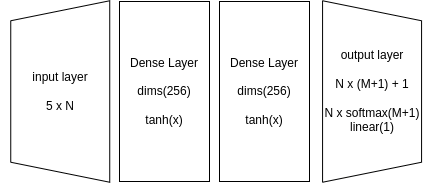
\includegraphics[width=\linewidth]{images/model_arch.png}
  \caption{Model architecture.}
  \label{fig:model}
\end{figure}

\section{Results}
\label{sec:results}
The code for the simulator, baselines and agent, as well as environment configurations, can be found in the following code repository: \hyperbf{https://github.com/Carlos-Marques/rl-MEC-scheduler}.

\subsection{Baselines} \label{baselines}
\noindent In order to benchmark the various \acrshort{DRL} algorithms and test the implemented simulator, several baseline algorithms were developed:

\begin{itemize}
    \item Full Local: all \acrshort{UE}s execute their tasks locally, in terms of the decision vector $\mathcal{A}=[0_1, 0_2, ..., 0_N]$. This represents the case where the system has no offloading capabilities.
    \item Random Offload: where the offloading decision is completely random, each task is either executed locally or offloaded to one of the available \acrshort{MEC} servers randomly;
    \item Full nearest \acrshort{MEC}: all \acrshort{UE} tasks are offloaded to the nearest \acrshort{MEC} server according. This represents the case of offloading to the nearest node without regarding their computation constraints and other offloading decisions. This baseline also requires knowledge of the network topology, which the agent does not have.
\end{itemize}

The plan is to create several system configurations of increasing complexity. The baseline algorithms will be used in order to benchmark the quality of trained agents. It is expected that the proposed network manager will surpass their performance in all situations by making intelligent decisions taking into account computation, battery, delay and communication constraints, which are ignored by the baselines.

\subsection{Simple test} \label{simple_test}

In order to put these baselines, the agent and the simulator to the test, a simple test case was devised. In this test, there are five \acrshort{UE}s and five \acrshort{MEC} servers. The UEs and MEC servers were randomly distributed in a 2D plane with $x \in [0, 200]$ and $y \in [0, 200]$, resulting in the distribution seen in Figure \ref{example_layout}.

\begin{figure}[H]
  \centering
  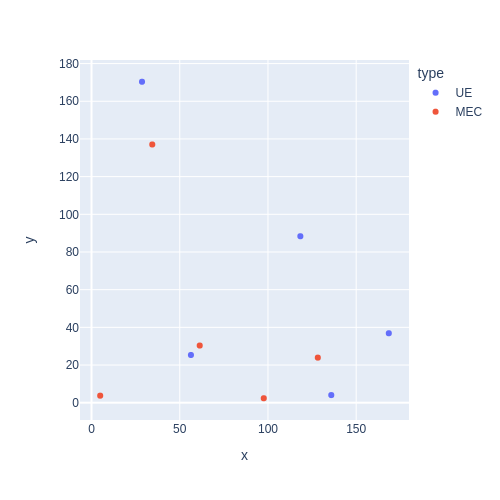
\includegraphics[width=200px]{images/example_layout.png}
  \caption{Example layout for the simple test.}  \label{example_layout}
\end{figure}

For simplicity, all \acrshort{UE}s and \acrshort{MEC} servers are considered to have the same specifications. The system's hyper-parameters were set according to the values present in Table \ref{hyperparams}. In order to test this configuration, the task parameters, $B_n$, $B_d$ and $D_n$ were sampled from uniform distributions between ($300$, $500$) Kbits, ($10$, $15$) Kbits and ($900$, $1100$) Megacyles, respectively. 

% Please add the following required packages to your document preamble:
% \usepackage[normalem]{ulem}
% \useunder{\uline}{\ul}{}
\begin{table}[H]
\centering
\begin{tabular}{|l|l|l|l|}
\hline
Variable             & Value & Variable                & Value \\ \hline
$B$&$10\times10^{6}$&$f_n^l$&$1\times10^{9}$\\
$n$&$10$&$I_n^t$&$0.5$\\
$\beta$&$-4$&$I_n^e$&$0.5$\\
$h_ul$&$100$& $P_m$&$200$\\
$h_dl$&$100$& $P_n$& $500\times10^{-3}$\\
$g_ul$&$1$&$P_n^i$&$100\times10^{-3}$\\
$g_dl$&$1$&$P_n^d$&$200\times10^{-3}$\\
$N_0$&$5\times10^{-5}$&$F_m$&$5\times10^{9}$\\
$W_{mean}$&$1$&$W_{max}$&$0$\\ \hline
\end{tabular}
\caption{System hyper-parameters.}\label{hyperparams}
\end{table}

The agent described in Section \ref{solution} was trained with the following hyper-parameters:

\begin{table}[H]
\centering
\begin{tabular}{|l|l|}
\hline
Variable & Value \\ \hline
episode length&$10$\\
learning rate, $\alpha$&$0.0001$\\
discount factor, $\gamma$&$0.99$\\
batch size&$200$\\ \hline
\end{tabular}
\caption{Training hyper-parameters.}\label{training_hyperparams}
\end{table}

Each algorithm ran for 100 episodes and an average per episode of offloading decisions is shown in Table \ref{resultstest1}.

\begin{table}[H]
\centering
\begin{tabular}{|l|l|l|}
\hline
Algorithm        & Average Reward ($R$) & Reduction\\ \hline
Full Local       & -49.47 & 96.65\%\\
Random Offload   & -9.68 & 82.89\%\\
Full nearest MEC & -2.18 & 24.06\%\\ 
Agent (A2C) & -1.66 & -\\ \hline
\end{tabular}
\caption{Results of simple test.} \label{resultstest1}
\end{table}

As expected, the Full Local baseline performed the worst given that it does not make use of the \acrshort{MEC} servers computing capabilities, leading to an increased cost due to increased energy consumption and delay of the tasks. The Random Offload baseline is the second worst, given that although it gains from offloading to \acrshort{MEC} servers, it does so without any consideration for the system's configuration. From the baselines, Full nearest MEC performed the best since it takes into consideration the distance between the \acrshort{UE} and the \acrshort{MEC} server. However, it comes with the disadvantage of not only requiring knowledge of the network topology (positions of \acrshort{UE}s and \acrshort{MEC}s) but also not taking into account anything else. 

As expected, the proposed agent outperformed the baselines in all situations, which demonstrates that the agent is able to learn not only the topology of the network by trying out different offloading decisions but also make intelligent decisions based on computation, battery, delay and communication constraints ignored by the baselines.

\begin{figure}[H]
  \centering
  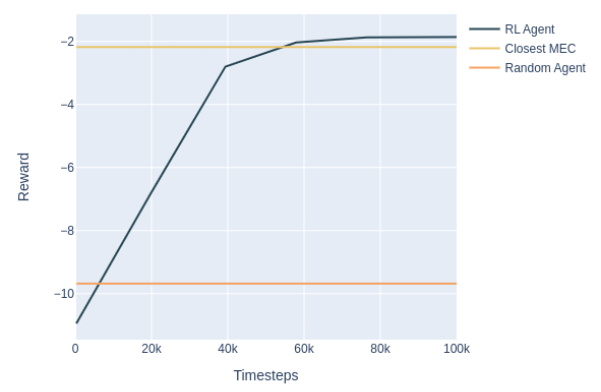
\includegraphics[width=\linewidth]{images/5_5_training.png}
  \caption{Agent reward while training.}  \label{5_5_training}
\end{figure}

As shown in Figure \ref{5_5_training}, the agent starts with an equivalent reward to the Random Offload, which is expected since the agent has not yet learned the environment. As the agent interacts with the environment making offloading decisions (actions), it receives state transitions and rewards. This allows it to quickly learn the system and the reward increases rapidly in the first iterations. After about 55K steps in the environment, the agent surpasses the best offloading baseline, Full nearest MEC. As expected, the reward starts to stabilize as the agent learns the final details of the system increasing slightly the final performance.

\subsection{Scalability and Data Efficiency} \label{scalability_data}

In this section, the scalability and data efficiency of our agent is explored. Scalability in this context can be defined as the ability of the agent to learn and outperform the baselines in higher complexity problems. 

Data efficiency in this context can be defined as the ability of the agent to learn in as few possible steps as possible. While it is expected that the agent takes longer to learn in more complex problems, the complexity of the underlying policy should not grow linearly with the state and action spaces. The reason for this is that it is expected that the agent is able to generalize concepts instead of brute forcing a solution for each problem set.

Since our state space is defined as the requested tasks at each step and each task is defined by a set of 5 parameters, the complexity of the state space grows linearly with the amount of \acrshort{UE}s, \emph{N}. The size of the state space should be $N \times 5$. 

On the other side, the action space is defined as the offloading decision of each task. Given that each task can be computed locally or offloaded to one of the \acrshort{MEC} servers, \emph{M}, this gives us the option of $M + 1$ actions per task. This results in the action space growing exponentially with the amount of \acrshort{UE}s, \emph{N}, since there are $(M + 1)^N$ possible actions at each decision step.

With this in mind, the stability and data efficieny of the system can be tested by setting the system's hyper-parameters and amount of \acrshort{MEC} servers to be the same as in the simple test case and create two new test scenarios by increasing the number of \acrshort{UE}s to 10 and 20, respectively.

The UEs and MEC servers were randomly distributed in a 2D plane with $x \in [0, 200]$ and $y \in [0, 200]$, resulting in the distribution seen in Figure \ref{5_10_layout} and Figure \ref{5_20_layout}.

\begin{figure}[H]
  \centering
  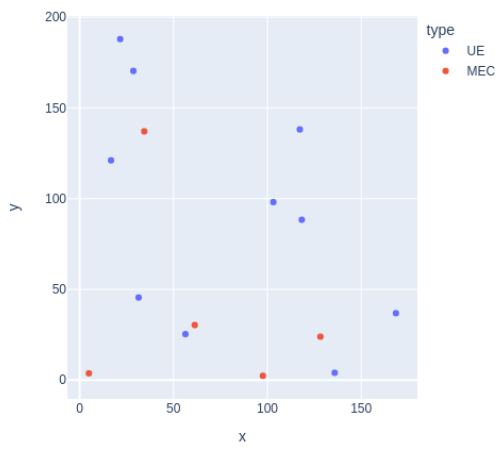
\includegraphics[width=200px]{images/5_10_layout.png}
  \caption{Test with 10 \acrshort{UE}s.}  \label{5_10_layout}
\end{figure}
\begin{figure}[H]
  \centering
  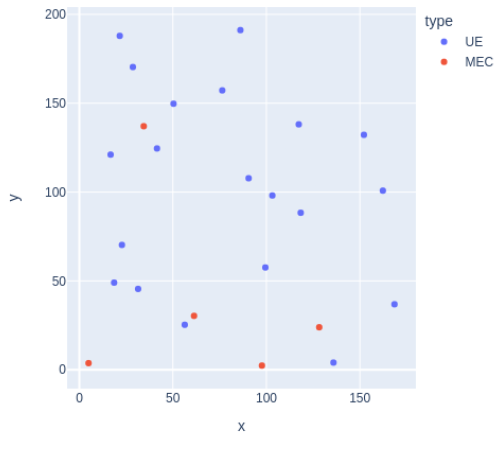
\includegraphics[width=200px]{images/5_20_layout.png}
  \caption{Test with 20 \acrshort{UE}s.}  \label{5_20_layout}
\end{figure}

Each algorithm ran for 100 episodes and an average per episode of offloading decisions is shown in Table \ref{results_5_10} and Table \ref{results_5_20}.

\begin{table}[H]
\centering
\begin{tabular}{|l|l|l|}
\hline
Algorithm        & Average Reward ($R$) & Reduction\\ \hline
Full Local       & -49.50 & 94.40\%\\
Random Offload   & -10.32 & 73.14\%\\
Full nearest MEC & -3.56 & 22.17\%\\ 
Agent (A2C) & -2.77 & -\\ \hline
\end{tabular}
\caption{Test results with 10 \acrshort{UE}s} \label{results_5_10}
\end{table}

\begin{table}[H]
\centering
\begin{tabular}{|l|l|l|}
\hline
Algorithm        & Average Reward ($R$) & Reduction\\ \hline
Full Local       & -49.49 & 90.42\%\\
Random Offload   & -11.67 & 59.36\%\\
Full nearest MEC & -7.23 & 34.38\%\\ 
Agent (A2C) & -4.74 & -\\ \hline
\end{tabular}
\caption{Test results with 20 \acrshort{UE}s} \label{results_5_20}
\end{table}

As expected, the reward of the Full Local baseline stays almost the same between test environments. This happens because these tests set $W_{mean}$ to 1 and $W_{max}$ to 0, so the cost is only composed by $C_{mean}$, defined in Equation \ref{C_mean}. Since $C_{mean}$ is the average cost of each \acrshort{UE}'s task, this should not scale with the amount of \acrshort{UE}s.

The same cannot be said of the other baselines and the agent. Since the number of \acrshort{MEC}s stays the same and the number of tasks increases, the overall cost of the system increases with the amount of \acrshort{UE}s. This represents the computation constraint of the \acrshort{MEC} servers. 

These results demonstrate that the agent scales with the complexity of the system.

In order to study the data efficiency of the agent, the agent's performance while training must be analysed.


\begin{figure}[H]
  \centering
  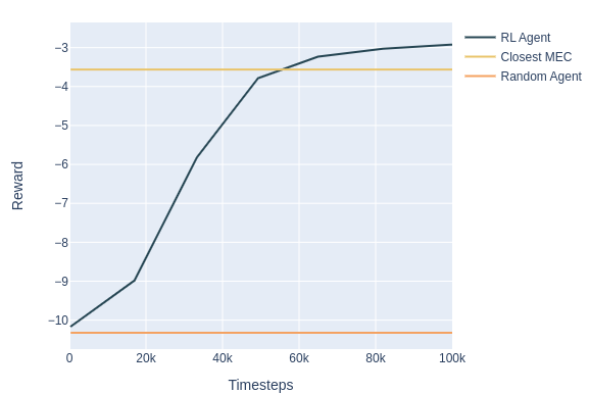
\includegraphics[width=\linewidth]{images/5_10_training.png}
  \caption{Training with 10 \acrshort{UE}s.}  \label{5_10_training}
\end{figure}
\begin{figure}[H]
  \centering
  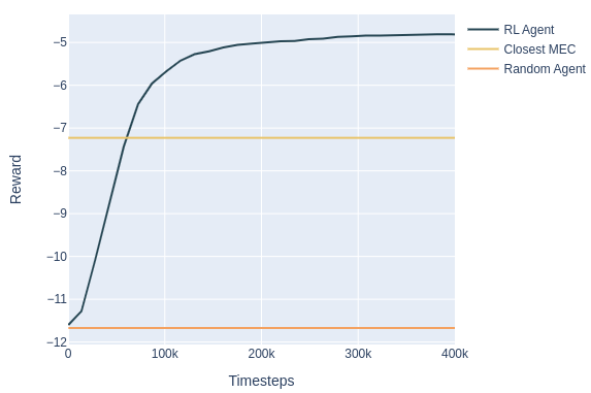
\includegraphics[width=\linewidth]{images/5_20_training.png}
  \caption{Training with 20 \acrshort{UE}s.}  \label{5_20_training}
\end{figure}

The same trend as the simple test can be observed with the two new tests in Figure \ref{5_10_training} and Figure \ref{5_20_training}.

This confirms that the agent is data efficient, meaning that even when the system's state space increases linearly and the action space increases exponentially, the agent is able to generalize concepts achieving a good performance. It does this with almost the same number of interactions with the system, proving it is finding a strategy without brute forcing a solution.

\subsection{Robustness and Stability} \label{robustness_stability}

In this section, the robustness and stability of our agent is explored. Robustness in this context can be defined as the ability of the agent to learn and outperform the baselines in environments with different network conditions and heterogeneous computation capabilities. 

Stability in this context can be defined has the ability of the agent to not diverge or collapse while training. This means that its performance should improve as it interacts with the environment, and after learning a strategy it should not forget it, collapsing the system's performance.

In order to test the system's robustness to changing network conditions, a new test case is devised by setting the system hyper-parameters to the values present in Table \ref{new_hyperparams}.

\begin{table}[H]
\centering
\begin{tabular}{|l|l|l|l|}
\hline
Variable             & Value & Variable                & Value \\ \hline
$B$&$10\times10^{6}$&$f_n^l$&$0.75\times10^{9}$\\
$n$&$10$&$I_n^t$&$0.25$\\
$\beta$&$-4$&$I_n^e$&$0.75$\\
$h_ul$&$50$& $P_m$&$100$\\
$h_dl$&$50$& $P_n$& $250\times10^{-3}$\\
$g_ul$&$0.5$&$P_n^i$&$50\times10^{-3}$\\
$g_dl$&$0.5$&$P_n^d$&$100\times10^{-3}$\\
$N_0$&$3\times10^{-5}$&$F_m$&$2.5\times10^{9}$\\
$W_{mean}$&$1$&$W_{max}$&$0$\\ \hline
\end{tabular}
\caption{New system hyper-parameters.}\label{new_hyperparams}
\end{table}

By setting the number of \acrshort{UE}s to 10 and the number of \acrshort{MEC}s to 5, they were randomly distributed in a 2D plane with $x \in [0, 200]$ and $y \in [0, 200]$, resulting in the distribution seen in Figure \ref{robust_test}.

\begin{figure}[H]
  \centering
  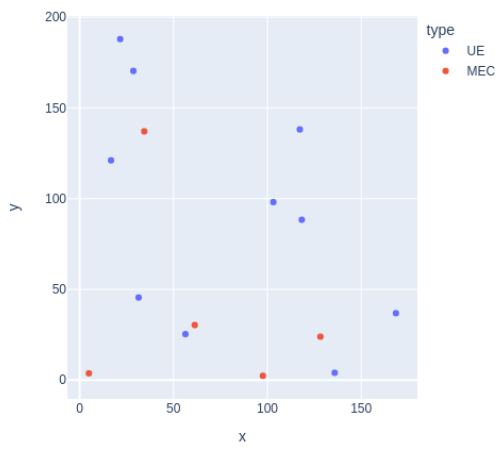
\includegraphics[width=200px]{images/5_10_layout.png}
  \caption{Robustness test layout.}  \label{robust_test}
\end{figure}

Each algorithm ran for 100 episodes and an average per episode of offloading decisions is shown in Table \ref{robust_table}.

\begin{table}[H]
\centering
\begin{tabular}{|l|l|l|}
\hline
Algorithm        & Average Reward ($R$) & Reduction\\ \hline
Full Local       & -31.31 & 84.92\%\\
Random Offload   & -9.14 & 48.35\%\\
Full nearest MEC & -6.81 & 30.62\%\\ 
Agent (A2C) & -4.72 & -\\ \hline
\end{tabular}
\caption{Robustness test results.} \label{robust_table}
\end{table}

As expected, the reward values of all the algorithms differ from previous tests since the system hyper-parameters that are used to calculate the reward function are different.

The same cost reduction trends can be observed in this new environment, showing that the agent is able to learn the system's behaviour independently of the network conditions.

\begin{figure}[H]
  \centering
  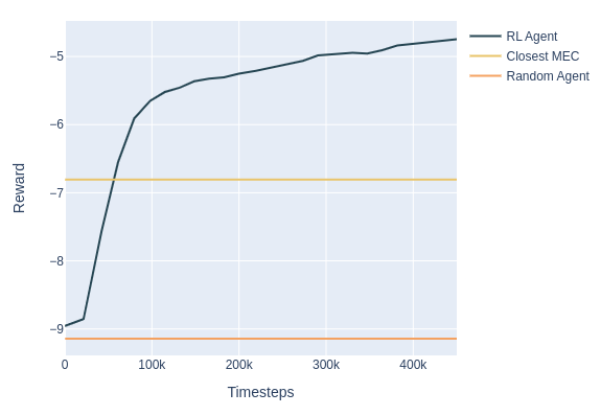
\includegraphics[width=\linewidth]{images/5_10_training_new.png}
  \caption{Training in robustness test.}  \label{robust_training}
\end{figure}

As shown in Figure \ref{robust_training}, the agent's performance while training follows a similar trend to previous tests.

The other component of robustness that must be tested is robustness to heterogeneous computation capabilities of \acrshort{UE}s and \acrshort{MEC} servers. To test this, a new test case is devised by resetting the system hyper-parameters to the values present in Table \ref{hyperparams} but instead of setting $f^l_n$ and $F_m$ to a fixed value, they are set to a value randomly sampled from a set of values, $f = \{0.25, 0.5, 0.75, 1\} \times 10^9$ and $F = \{2.5, 5, 7, 10\} \times 10^9$, respectively.

By setting the number of \acrshort{UE}s to 10 and the number of \acrshort{MEC}s to 5, they were randomly distributed in a 2D plane with $x \in [0, 200]$ and $y \in [0, 200]$, resulting in the distribution seen in Figure \ref{hetero_test}.

\begin{figure}[H]
  \centering
  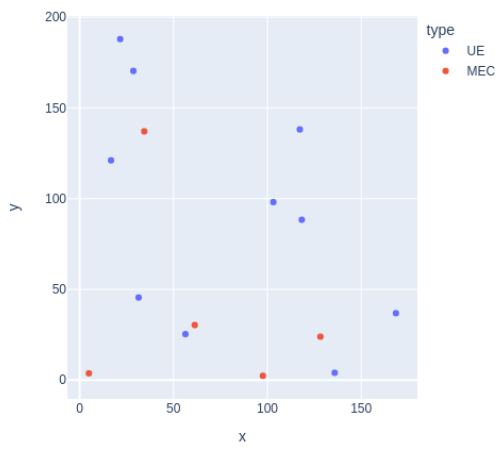
\includegraphics[width=200px]{images/5_10_layout.png}
  \caption{Heterogeneous test layout.}  \label{hetero_test}
\end{figure}

Each algorithm ran for 100 episodes and an average per episode of offloading decisions is shown in Table \ref{hetero_table}.

\begin{table}[H]
\centering
\begin{tabular}{|l|l|l|}
\hline
Algorithm        & Average Reward ($R$) & Reduction\\ \hline
Full Local       & -33.56 & 89.55\%\\
Random Offload   & -8.80 & 60.16\%\\
Full nearest MEC & -5.04 & 30.39\%\\ 
Agent (A2C) & -3.51 & -\\ \hline
\end{tabular}
\caption{Heterogeneous test results.} \label{hetero_table}
\end{table}

As presumed, the reward values of all the algorithms differ from previous tests since the system computation capabilities that are used to calculate the reward function are different.

Although the ordering of the algorithm performances stays the same in this test case, the cost reduction of our agent in comparison to the Full nearest MEC is higher. With a reported 30.39\% improvement, while the equivelant homogeneous test had an improvement of 22.17\%. This makes sense given that the Full nearest MEC only takes into account the distance of \acrshort{UE}s to \acrshort{MEC}s and not their computation capabilities. This, in turn, leads to worse load balancing when the computation capabilities of the \acrshort{UE}s and \acrshort{MEC}s are not all the same.

The agent on the other hand is able to learn the system's network topology and make offloading decisions that better load balance the required tasks. 

By analysing all training curves, it is clear that the agent is stable and its reward does not diverge or collapse while training, even when ran for millions of iterations.

\begin{figure}[H]
  \centering
  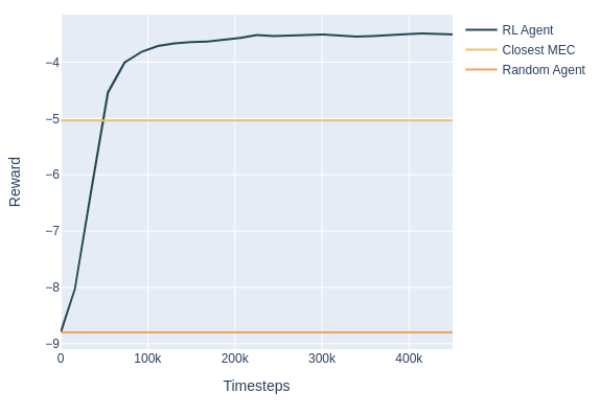
\includegraphics[width=250px]{images/5_10_training_hetero.png}
  \caption{Training in heterogeneous environment.}  \label{hetero_training}
\end{figure}

As shown in Figure \ref{hetero_training}, the agent's performance while training follows a similar trend to previous tests.

\subsection{Reward function weights} \label{reward_section}

This section focuses on studying the effect of the cost function importance weights on the agent's overall and worst-case performance.

To test this, five new test cases were created by setting the system hyper-parameters to the values present in Table \ref{hyperparams} but instead of setting $W_{mean}$ to 1 and $W_{max}$ to 0, they are set to $(1, 0.75, 0.5, 0.25, 0)$ and $(0, 0.25, 0.5, 0.75, 1)$, respectively.

By setting the number of \acrshort{UE}s to 10 and the number of \acrshort{MEC}s to 5, they were randomly distributed in a 2D plane with $x \in [0, 200]$ and $y \in [0, 200]$, resulting in the distribution seen in Figure \ref{weight_test}.

\begin{figure}[H]
  \centering
  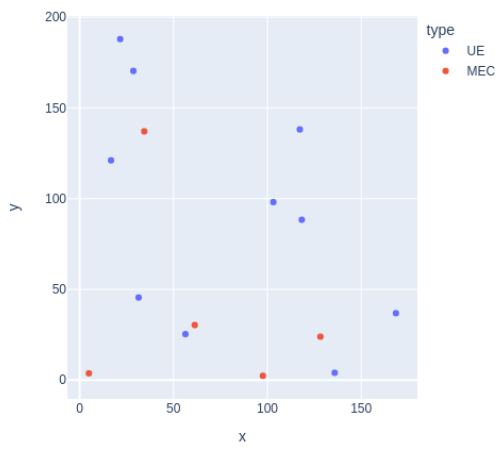
\includegraphics[width=200px]{images/5_10_layout.png}
  \caption{Weight test layout.}  \label{weight_test}
\end{figure}

Each combination of the cost function ran for 100 episodes and an average per episode of offloading decisions is shown in Table \ref{weight_table}.

\begin{table}[H]
\centering
\begin{tabular}{|l|l|l|l|}
\hline
$\{W_{mean}, W_{max}\}$ & Overall Cost & Worst Cost & Difference \\ \hline
$\{1, 0\}$       & 2.72 & 4.04 & 1.32\\
$\{0.75, 0.25\}$  & 2.97 & 3.84  & 0.87\\
$\{0.5, 0.5\}$ & 3.22 & 3.53 & 0.31\\ 
$\{0.25, 0.75\}$ & 3.52 & 3.81 & 0.29\\ 
$\{0, 1\}$ & 3.81 & 3.78 & -0.03 \\ \hline
\end{tabular}
\caption{Weight test results.} \label{weight_table}
\end{table}

As the weights shift from prioritizing overall performance to prioritizing worst-case performance, the agent's overall cost increases while the worst-case cost decreases. While the agent outperforms the best baseline with every weight distribution, it learns to make offloading decisions that prioritize the worst-case performance at the expense of overall system performance. With this in mind, the process of picking the best weight distribution would involve trying to determine the maximum cost allowed per \acrshort{UE} and shifting the weight distribution in favour of $W_{max}$, trying to maximize $W_{mean}$ while still meeting the maximum allowed cost.




\section{Conclusion}
\label{sec:conclusion}

\subsection{Summary}
\noindent As presented in Section \ref{section:MECarch} several architectures have been proposed in the \acrshort{MEC} context that present complex optimization problems of managing how to distribute tasks between \acrshort{UE}s and \acrshort{MEC} servers. Due to the high dimensional complexity and uncertain networking conditions, classical offline optimization algorithms fail to effectively manage these types of problems. Based on the work done by papers \cite{taskclass1} and \cite{NUE1mec} a more complete system that takes into account the possibility of offloading between a network of heterogeneous \acrshort{UE}s to a network of heterogeneous \acrshort{MEC} servers is proposed. As far as the candidate knows, this is the first time this extended optimization problem is addressed. In order to deal with the increased complexity of taking into account computation, battery, delay and communication constraints in an \emph{N} to \emph{N} problem, a network manager agent is proposed in Section \ref{solution}. In order to evaluate the performance of the proposed agent, several baselines are described in Section \ref{baselines}. Finally, the agent's capabilities are put to the test in Sections \ref{simple_test}, \ref{scalability_data}, \ref{robustness_stability} and \ref{reward_section}. The proposed agent is shown to be scalable, data-efficient, robust, stable and adjustable to address not only overall system performance but to take into account the worst-case scenario.

\subsection{Future Work}
\noindent Future steps of research should include:
\begin{itemize}
    \item Expanding the proposed simulator to include more dynamic environments, implementing the ability to change the following as simulation progresses:
    \begin{itemize}
      \item \acrshort{UE} locations to simulate mobility;
      \item The number of \acrshort{UE}s and \acrshort{MEC} servers;
      \item Network conditions.
    \end{itemize}
    \item Creating a more complete test set, testing environments for specific scenarios. For example, a Smart city environment or an autonomous vehicle environment. 
    \item Exploring the use of this orchestration agent with choreography algorithms like the one proposed in \cite{Lulu}, by simulating an environment where several groups of \acrshort{MEC} servers would be orchestrated by agents like the one proposed in this work, while choreographing with each other.
    \item Exploring the use of model based \acrshort{RL} algorithms to take advantage of the extensive domain knowledge of telecommunication physics. By leveraging this knowledge, the agent could converge to a better solution more quickly without having to learn this through experimentation.
\end{itemize}


\begin{thebibliography}{1}

\bibitem{SHAKARAMI2020107496}
A.~Shakarami, M.~Ghobaei-Arani, and A.~Shahidinejad, ``A survey on the
  computation offloading approaches in mobile edge computing: A machine
  learning-based perspective,'' {\em Computer Networks}, vol.~182, p.~107496,
  2020.

\bibitem{MECspec}
M.~Patel, B.~Naughton, C.~Chan, N.~Sprecher, S.~Abeta, A.~Neal, {\em et~al.},
  ``Mobile-edge computing introductory technical white paper,'' {\em White
  paper, mobile-edge computing (MEC) industry initiative}, vol.~29,
  pp.~854--864, 2014.

\bibitem{opengym}
G.~Brockman, V.~Cheung, L.~Pettersson, J.~Schneider, J.~Schulman, J.~Tang, and
  W.~Zaremba, ``Openai gym,'' {\em CoRR}, vol.~abs/1606.01540, 2016.

\bibitem{cloudlet}
M.~Satyanarayanan, P.~Bahl, R.~Caceres, and N.~Davies, ``The case for vm-based
  cloudlets in mobile computing,'' {\em IEEE Pervasive Computing}, vol.~8,
  no.~4, pp.~14--23, 2009.

\bibitem{adhoc}
G.~A. McGilvary, A.~Barker, and M.~Atkinson, ``Ad hoc cloud computing,'' in
  {\em 2015 IEEE 8th International Conference on Cloud Computing},
  pp.~1063--1068, 2015.

\bibitem{smallcellcloud}
F.~Lobillo, Z.~Becvar, M.~A. Puente, P.~Mach, F.~Lo~Presti, F.~Gambetti,
  M.~Goldhamer, J.~Vidal, A.~K. Widiawan, and E.~Calvanesse, ``An architecture
  for mobile computation offloading on cloud-enabled lte small cells,'' in {\em
  2014 IEEE Wireless Communications and Networking Conference Workshops
  (WCNCW)}, pp.~1--6, 2014.

\bibitem{mmcloud}
S.~Wang, G.-H. Tu, R.~Ganti, T.~He, K.~Leung, H.~Tripp, K.~Warr, and M.~Zafer,
  ``Mobile micro-cloud: Application classification, mapping, and deployment,''
  in {\em Proc. Annual Fall Meeting of ITA (AMITA)}, 2013.

\bibitem{MobiScud}
K.~Wang, M.~Shen, J.~Cho, A.~Banerjee, J.~K.~V. der Merwe, and K.~Webb,
  ``{MobiScud:} a fast moving personal cloud in the mobile network,'' 2015.

\bibitem{fmcloud}
A.~Aissioui, A.~Ksentini, and A.~Gueroui, ``An efficient elastic distributed
  sdn controller for follow-me cloud,'' in {\em 2015 IEEE 11th International
  Conference on Wireless and Mobile Computing, Networking and Communications
  (WiMob)}, pp.~876--881, 2015.

\bibitem{CONCERT}
J.~Liu, T.~Zhao, S.~Zhou, Y.~Cheng, and Z.~Niu, ``Concert: a cloud-based
  architecture for next-generation cellular systems,'' {\em IEEE Wireless
  Communications}, vol.~21, no.~6, pp.~14--22, 2014.

\bibitem{SESAM}
H.~E. Project, ``Small cells coordination for multi-tenancy and edge services
  (sesam)..'' Online, 2015.
\newblock Last access on 28/05/2021.

\bibitem{DQN}
V.~Mnih, K.~Kavukcuoglu, D.~Silver, A.~A. Rusu, J.~Veness, M.~G. Bellemare,
  A.~Graves, M.~Riedmiller, A.~K. Fidjeland, G.~Ostrovski, S.~Petersen,
  C.~Beattie, A.~Sadik, I.~Antonoglou, H.~King, D.~Kumaran, D.~Wierstra,
  S.~Legg, and D.~Hassabis, ``Human-level control through deep reinforcement
  learning,'' {\em Nature}, vol.~518, pp.~529--533, Feb 2015.

\bibitem{doubleDQN}
H.~v. Hasselt, ``Double q-learning,'' in {\em Proceedings of the 23rd
  International Conference on Neural Information Processing Systems - Volume
  2}, NIPS'10, (Red Hook, NY, USA), p.~2613–2621, Curran Associates Inc.,
  2010.

\bibitem{duelingDQN}
Z.~Wang, N.~de~Freitas, and M.~Lanctot, ``Dueling network architectures for
  deep reinforcement learning,'' {\em CoRR}, vol.~abs/1511.06581, 2015.

\bibitem{a3c}
V.~Mnih, A.~P. Badia, M.~Mirza, A.~Graves, T.~P. Lillicrap, T.~Harley,
  D.~Silver, and K.~Kavukcuoglu, ``Asynchronous methods for deep reinforcement
  learning,'' {\em CoRR}, vol.~abs/1602.01783, 2016.

\bibitem{boltz}
N.~Cesa{-}Bianchi, C.~Gentile, G.~Lugosi, and G.~Neu, ``Boltzmann exploration
  done right,'' {\em CoRR}, vol.~abs/1705.10257, 2017.

\bibitem{AGAcrypto}
X.~Qiu, L.~Liu, W.~Chen, Z.~Hong, and Z.~Zheng, ``Online deep reinforcement
  learning for computation offloading in blockchain-empowered mobile edge
  computing,'' {\em IEEE Transactions on Vehicular Technology}, vol.~68, no.~8,
  pp.~8050--8062, 2019.

\bibitem{taskclass1}
Y.~Gong, C.~Lv, S.~Cao, L.~Yan, and H.~Wang, ``Deep learning-based computation
  offloading with energy and performance optimization,'' {\em EURASIP Journal
  on Wireless Communications and Networking}, vol.~2020, p.~69, Mar 2020.

\bibitem{Lulu}
L.~P. de~Matos Morgado~Ferreira, ``Fog computing task offloading optimization
  based on deep reinforcement learning,'' Master's thesis, Instituto Superior
  Técnico, 2021.

\bibitem{NUE1mec}
J.~Li, H.~Gao, T.~Lv, and Y.~Lu, ``Deep reinforcement learning based
  computation offloading and resource allocation for mec,'' in {\em 2018 IEEE
  Wireless Communications and Networking Conference (WCNC)}, pp.~1--6, 2018.

\bibitem{energycons}
Y.~Wen, W.~Zhang, and H.~Luo, ``Energy-optimal mobile application execution:
  Taming resource-poor mobile devices with cloud clones,'' in {\em 2012
  Proceedings IEEE INFOCOM}, pp.~2716--2720, 2012.

\end{thebibliography}

\end{document}
